%%%%%%%%%%%%%%%%%%%%%%%%%%%%%%%%%%%%%%%%%%%%%%
%       Plantilla Informes Isaias Cardenas
%%%%%%%%%%%%%%%%%%%%%%%%%%%%%%%%%%%%%%%%%%%%%%

\documentclass[letterpaper,12pt]{report}
\usepackage[right=2cm,left=3cm,top=2cm,bottom=2cm,footskip=1.4cm]{geometry}%margenes de la pagina

\usepackage{ucs}
\usepackage[utf8x]{inputenc}
\usepackage[spanish, es-tabla]{babel}
\usepackage[T1]{fontenc}
\usepackage{blindtext}
\usepackage{enumitem}
\usepackage{graphicx}
\usepackage{listings} % escribir codigo
\usepackage{algpseudocode} % escribir algoritmos
\graphicspath{ {./images/} }
\usepackage{multicol} % multicolumnas
% \usepackage{subfigure} % incluir multiples imágenes en una figura
\usepackage{float} % poscicionar imagenes

% \RequirePackage{hyperref}
% \RequirePackage{url} %citacion de URL
% \usepackage{hyperref}
\linespread{1.5} %interlineado

%borra la palabra "capitulo"
\usepackage{titlesec}
\titleformat{\chapter}[display]
    {\normalfont\huge\bfseries}{}{0pt}{\Huge}
\titlespacing*{\chapter}
    {0pt}{10pt}{40pt}


\begin{document}
\renewcommand{\contentsname}{Tabla de Contenido}
\begin{titlepage}
\begin{center}
UNIVERSIDAD DE SANTIAGO DE CHILE\\
FACULTAD DE INGENIERÍA\\
DEPARTAMENTO DE INGENIERÍA INFORMÁTICA\\
\begin{figure}[htb]
\begin{center}

\includegraphics[width=4.5cm]{logo.png}
\end{center}
\end{figure}

\vspace*{0.7in}
\begin{Large}
\textbf{Entrega 1: Buscaminas} \\
\end{Large}
\vspace*{0.3in}

\vspace*{2in}

\end{center}
\begin{flushright}

\begin{tabular}{lll}
Alumno & : & Isaías Cárdenas\\
Rut & : & 18750177-6\\
Profesor & : & Pablo Schwarzenberg\\
Curso & : & Laboratorio estructura de datos y análisis de algoritmos\\
Ayudantes & : & Sebastián Vallejos\\
          &  & Javiera Torres\\
Fecha de entrega & : & 30 de agosto de 2017
\end{tabular}
\end{flushright}
\end{titlepage}

\tableofcontents

\chapter{Introducci\'on}

\section {Introducci\'on al problema}

El presente proyecto consiste en crear un programa que simule el juego ``Buscaminas''. El juego, al igual que en su modalidad clásica, consta de un tablero que tiene bombas escondidas en algunas casillas y de pistas colocadas en casillas adyacentes a las bombas; el objetivo del jugador es encontrar todas las bombas escondidas en el tablero sin hacerlas ``estallar'', para ello puede marcar las casillas que él crea que contengan bombas. Las acciones permitidas al usuario serán ``O'' para revelar una casilla y ``X'' para marcar una casilla con posible bomba. El tamaño y la cantidad de bombas serán escogidos por el jugador de manera que es él quien decida la dificultad del juego. Además de la jugabilidad principal el alumno deberá generar un archivo con el contenido del tablero a modo de solución del juego. Para implementar éste programa el alumno deberá utilizar el lenguaje de programación C en su versión estándar (ANSI C).

\chapter{Descripci\'on del problema}

\section {Descripci\'on del problema}

A partir de la jugabilidad principal del Buscaminas se desprenden subproblemas mas básicos que en conjunto resuelven el problema general, lo primero sería realizar un tablero a partir de los datos ingresados por el usuario. El tablero debe tener casillas con el contenido oculto al usuario; este contenido puede ser una pista (número), una bomba, o simplemente vacío. El contenido de la casilla puede ser revelado al usuario si él realiza la acción ``O'' en ella, por otro lado el usuario debe poder marcar una casilla si realiza la acción ``X'' en ella. El ingreso de acciónes del usuario deben tener el formato:

\begin{lstlisting}[language=bash]
<< coordenada horzontal, coordenada vertical, accion >>
\end{lstlisting}

Tal y como se muestra en el ejempo de la figura \ref{fig:ejemploEntrada}.

\begin{figure}[H]
    \centering
    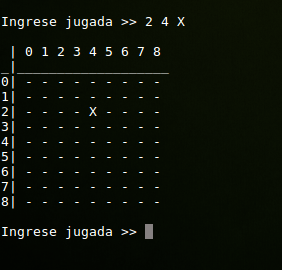
\includegraphics[width=0.4\textwidth]{ejemploEntrada.png}
    \caption{Ejemplo de una entrada del usuario}
    \label{fig:ejemploEntrada}
\end{figure}

Cada bomba debe estar rodeada de mas bombas o de pistas que le muestran al usuario cuantas bombas hay al rededor. En el tablero las pistas son representadas por un número que indican cuantas bombas rodean la casilla en la que se encuentra la pista, a modo de ejemplo la figura \ref{fig:ejemploPista} muestra como se vería una pista en el tablero.

\begin{figure}[H]
    \centering
    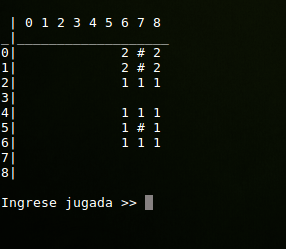
\includegraphics[width=0.4\textwidth]{ejemploPista.png}
    \caption{Ejemplo de una pista en el tablero}
    \label{fig:ejemploPista}
\end{figure}

Si la casilla que desea revelar el jugador esta vacía se deben revelar las casillas contiguas a ésta (adyacentes y diagonales) hasta que se encuentre una pista o una bomba, en este último caso la casilla no debe ser revelada. Si el usuario revela una casilla con una bomba pierde el juego por lo que el tablero no debe contener bombas hasta que el jugador realize la primera accion de modo que nunca pueda perder en la primera jugada. El juego termina si el usario revela todas las casillas que no contengan bombas ganando la partida, o si revela una bomba perdiendo el juego.

Adicional a la jugabilidad se debe generar un archivo llamado ``solucion.out'' que contenga el tablero completamente revelado, este archivo debe crearse luego de la primera jugada del usuario.

\chapter{Descripci\'on de la soluci\'on}

\section {Marco te\'orico}

Para una mejor comprensión de la descripción de la solución es preciso definir algunos conceptos que
serán indispensables en éste proyecto:

\begin{description}[align=left]

\item [Programaci\'on imperativa:] 
    La programación imperativa es un paradigma de programación que se basa en que los programas 
    deben darle una serie de instrucciones al computador que describan como realizar una tarea,
    dicho de otro modo, este paradigma busca emular el modo imperativo del lenguaje humano. 

\item [Punteros:]
    Los punteros son objetos utilizados en la programaci\'on para referirse o apuntar a algún valor almacenado
    en memoria usando su ubicación, de manera que los valores no necesariamiente deben ser contiguos en memoria.
    El uso de punteros en un lenguaje de programación mejora significativamente el rendimiento de un programa que 
    manipule la información con estructuras de datos (tipos de datos abstractos) y con ello la eficiencia de éste.

\item [Estructura:]
    Una estructura es un conjunto de variables de tipo de datos básico agrupadas en una estructura lógica, esta estructura puede ser utilizada varias veces como un tipo de dato compuesto. El lenguaje C permite la definición de estructuras a fin de facilitar la producción de código al programador.

\item [Lenguaje de programaci\'on ANSI C:]
    El lenguaje C es un lenguaje de programación imperativo estructural caracterizado por
    posibilitar la manipulación de memoria a través de punteros. C es uno de los lenguajes más
    utilizados en el desarrollo de software de sistemas dado que su eficiencia en código es 
    muy alta. El instituto nacional estadounidense de estandarés publicó un estándar para el 
    lenguaje C de manera que a los desarrolladores se les facilitara la portabilidad del código,
    éste estándar fue llamado ANSI C.

\end{description}

\section {Herramentas y técnicas}

Para la implementación de este proyecto se utilizaron en general 2 técnicas de la programación con el fin de facilitar la resolución de problemas puntuales, o subproblemas del proyecto:

\begin{description}[align=left]

\item [Iteración:]
    Las iteraciones hacen referencia a una serie de pasos, o instrucciones, que el computador debe realizar según una o varias condiciones. En general esta técnica es muy básica y es ampliamente utilizada en la programación, es común realizar combinaciones con otras técnicas de manera iterativa e incluso anidar iteraciónes.

\item [Recursividad:] 
    Es una técnica que consiste en crear un proceso(o función) que se llama a sí mismo, es decir, el proceso se espesifica basandose en su propia definición. La recursividad es utilizada para reemplazar procesos iterativos que podrían tener una codificación mas extensa.

\end{description} 

En general y a modo de herramientas externas se utilizaron las librerías estándar de ANSI C: ``stdio.h'' para las entradas y salidas estándares, ``stdlib.h'' para las utilidades generales en un script como la gestión de la memoria dinámica, función rand() para números aleatorios, casteo de variables, etc; y ``string.h'' para el manejo de strings en c.

Dado a que C es un lenguaje imperativo y estructural se hicieron uso de estructuras para ordenar la información y así facilitar el orden lógico a quien quiera leer e interpretar el código, haciendo mas semántico el uso de las variables. La definición y descripición de  estas estructuras se detallan en la siguiente sección.

\section {Algoritmos y estructuras}

Para generar el tablero se crearán 2 estructuras principales: BoardBlock y Board, para las casillas y el tablero respectivamente. La interacción entre estas estructuras realizará la jugabilidad del buscaminas, de modo que la implementación en código sea mas ordenada. La estructura BoardBlock contiene los siguienes atributos:

\begin{figure}[H]
    \centering
    \begin{tabular}{|l|p{10cm}|}
        \hline
        Hidden & Entero que indica si la casilla tiene su contenido oculto al usuario, sus valores son ``1'' si su contenido esta oculto y ``0'' si no lo está.\\
        \hline
        Content & Carácter que representa el contenido de la casilla, sus valores pueden ser un número(pista), el carácter `` ' '' para indicar que la casilla esta vacia y el carácter `` * '' para representar que la casilla contiene una bomba.\\
        \hline
        Bomb & Entero que indica si la casilla contiene una bomba, sus valores son ``1'' si la casilla tiene una bomba y ``0'' en caso contrario.\\
        \hline
        Check & Entero que indica si la casilla esta marcada como posible bomba, sus valores pueden ser ``1'' si se encuentra marcada por el usuario y ``0'' si no lo está.\\
        \hline
    \end{tabular}
    \caption{Tabla atributos de la estructura BoardBlock}
    \label{table:BoardBlock}
\end{figure}

Luego se genera la estructura Board que contiene una matriz bidimencional utilizando a la estructura de figura \ref{table:BoardBlock}, te esta manera se realiza la jugabilidad del Buscaminas implementando solamente una matriz. La estructura Board consta de los siguientes atributos:

\begin{figure}[H]
    \centering
    \begin{tabular}{|l|p{10cm}|}
        \hline
        Rows & Entero que indica la cantidad de filas presentes en el tablero, su valor es ingresado por el usuario.\\
        \hline
        Columns & Entero que representa la cantidad de columnas que tiene el tablero, su valor es ingresado por el usuario.\\
        \hline
        Matrix & Puntero doble a la estructura BoardBlock, será utilizado para generar una matriz bidimencional que represente el tablero de juego de ``rows'' filas por ``columns'' columnas.\\
        \hline
    \end{tabular}
    \caption{Tabla atributos de la estructura Board}
    \label{table:Board}
\end{figure}

A partir de estas estructuras se generará el tablero de juego, de esta manera será necesario implementar solamente una matriz. Luego de inicializar las estructuras con los datos ingresados y de leer la primera jugada del usuario, se colocarán las bombas en el tablero de forma aleatoria, usando la función ``rand()'' de C, teniendo en cuenta de no posicionarla en la casilla en la que el usuario ha hecho su primera jugada. Con las bombas colocadas en el tablero bastará de recorrer casilla por casilla y contar la cantidad de bombas contiguas en cada una de ellas para obtener las pistas para el usuario. 

En caso de que el jugador quiera revelar una casilla vacia es necesario revelar todas las casillas contiguas a ésta hasta que la casilla contenga una pista o una bomba, para realizar este proceso se crea una función recursiva según el siguiente algoritmo:

\begin{figure}[p]
    \begin{algorithm}
    \Procedure{\textbf{function} unHide}{$board, x, y$}

        \If{x+1 > board.rows \textbf{or} y+1 > board.columns \textbf{or} x < 0 \textbf{or} y < 0}
            \State{\textbf{return} False;}
        \EndIf
        \If{is \textbf{not} board.table[x][y].hidden}
            \State{\textbf{return} False;}
        \ElsIf{is ``bomb'' == board.table[x][y].content}
            \State{board.table[x][y].hidden = False;}
            \State{\textbf{return} True;}
        \ElsIf{is \textbf{not} `` '' == board.table[x][y].content}
            \State{board.table[x][y].hidden = False;}
            \State{\textbf{return} False;}
        \EndIf

        \State{board.table[x][y].hidden = False;}
        \State{\textbf{return} unHide(board, x+1, y) \textbf{and}
        \State{unHide(board, x-1, y) \textbf{and}}
        \State{unHide(board, x, y+1) \textbf{and}}
        \State{unHide(board, x, y-1);} 
            
    \EndProcedure
    \end{algorithm}
    \caption{Algoritmo recursivo unHide}
    \label{algrthm:unhide}
\end{figure}

Con las funciones principales realizadas para la jugabilidad, hace falta verificar si el jugador gana o pierde. El usuario pierde la partida si revela una bomba, y gana si ha revelado todas las casillas que no contienen bombas por lo que es necesario contar las casillas que ha revelado.

Finalmente se escribe un archivo con el contenido de la matriz luego de la primera jugada del usuario, para ello simplemente se recorre la matriz y se escribe su contenido casilla a casilla en el archivo de salida. La jugabilidad principal se engloba en un ciclo iterativo que verifica en cada jugada si el usuario gana o pierde la partida.


\chapter{Conclusiones}

\section {An\'alisis de los resultados}

analisis de tiempos de ejecución

\section {Conclusiones}

Se cumplen los objetivos propuestos y los requerimientos solicitados en el plazo estipulado, el uso de punteros y el manejo de memoria dinámica se logra en totalidad logarando crear una matriz bidimencional que contiene estructuras. ...

\end{document}
